%UG project example file, February 2022
%   A minior change in citation, September 2023 [HS]
% Do not change the first two lines of code, except you may delete "logo," if causing problems.
% Understand any problems and seek approval before assuming it's ok to remove ugcheck.
\documentclass[logo,bsc,singlespacing,parskip]{infthesis}
\usepackage{ugcheck}

\usepackage{amsmath}
\usepackage{amsthm}
\usepackage{amssymb}
\usepackage{hyperref}
\usepackage{cleveref}
\usepackage{algorithm}
\usepackage{algpseudocodex}

\usetikzlibrary{calc,arrows.meta,positioning, bending}

\theoremstyle{definition}
\newtheorem{definition}{Definition}[section]

\theoremstyle{example}
\newtheorem{example}[definition]{Example}

\theoremstyle{theorem}
\newtheorem{prop}[definition]{Proposition}

\theoremstyle{theorem}
\newtheorem{lemma}[definition]{Lemma}

\theoremstyle{theorem}
\newtheorem{cor}[definition]{Corollary}

\theoremstyle{theorem}
\newtheorem{theorem}[definition]{Theorem}

\theoremstyle{definition}
\newtheorem{remark}[definition]{Remark}

\theoremstyle{definition}
\newtheorem{notation}[definition]{Notation}

\theoremstyle{definition}
\newtheorem{ex}[definition]{Example}

\renewcommand{\qedsymbol}{$\blacksquare$}
\newcommand{\znn}{\mathbb{Z}_{\geq 0}}
\newcommand{\trsk}{\textsc{Tarski}}
\newcommand{\nd}{[N]^d}
% \newcommand{\bot}{\text{bot}}
% \newcommand{\top}{\text{top}}
\newcommand{\mi}{\text{mid}}
\newcommand{\arr}{\textsc{Arrival}}

\newcommand\restr[2]{{
  \left.\kern-\nulldelimiterspace 
  #1 
  \littletaller
  \right|_{#2} 
  }}
  \newcommand{\littletaller}{\mathchoice{\vphantom{\big|}}{}{}{}}


% Include any packages you need below, but don't include any that change the page
% layout or style of the dissertation. By including the ugcheck package above,
% you should catch most accidental changes of page layout though.

\usepackage{microtype} % recommended, but you can remove if it causes problems
\usepackage{natbib} % recommended for citations

\begin{document}
\begin{preliminary}

\title{Tarski Fixed Point Computation and the Arrival Problem}

\author{Angus Joshi}

% CHOOSE YOUR DEGREE a):
% please leave just one of the following un-commented
% \course{Artificial Intelligence}
%\course{Artificial Intelligence and Computer Science}
%\course{Artificial Intelligence and Mathematics}
%\course{Artificial Intelligence and Software Engineering}
%\course{Cognitive Science}
%\course{Computer Science}
%\course{Computer Science and Management Science}
\course{Computer Science and Mathematics}
%\course{Computer Science and Physics}
%\course{Software Engineering}
%\course{Master of Informatics} % MInf students

% CHOOSE YOUR DEGREE b):
% please leave just one of the following un-commented
%\project{MInf Project (Part 1) Report}  % 4th year MInf students
%\project{MInf Project (Part 2) Report}  % 5th year MInf students
\project{4th Year Project Report}        % all other UG4 students


\date{\today}

\abstract{
This skeleton demonstrates how to use the \texttt{infthesis} style for
undergraduate dissertations in the School of Informatics. It also emphasises the
page limit, and that you must not deviate from the required style.
The file \texttt{skeleton.tex} generates this document and should be used as a
starting point for your thesis. Replace this abstract text with a concise
summary of your report.
}

\maketitle

\newenvironment{ethics}
   {\begin{frontenv}{Research Ethics Approval}{\LARGE}}
   {\end{frontenv}\newpage}

\begin{ethics}
This project was planned in accordance with the Informatics Research
Ethics policy. It did not involve any aspects that required approval
from the Informatics Research Ethics committee.

\standarddeclaration
\end{ethics}


\begin{acknowledgements}
Any acknowledgements go here.
\end{acknowledgements}


\tableofcontents
\end{preliminary}


\chapter{Introduction}

The preliminary material of your report should contain:
\begin{itemize}
\item
The title page.
\item
An abstract page.
\item
Declaration of ethics and own work.
\item
Optionally an acknowledgements page.
\item
The table of contents.
\end{itemize}

As in this example \texttt{skeleton.tex}, the above material should be
included between:
\begin{verbatim}
\begin{preliminary}
    ...
\end{preliminary}
\end{verbatim}
This style file uses roman numeral page numbers for the preliminary material.

The main content of the dissertation, starting with the first chapter,
starts with page~1. \emph{\textbf{The main content must not go beyond page~40.}}

The report then contains a bibliography and any appendices, which may go beyond
page~40. The appendices are only for any supporting material that's important to
go on record. However, you cannot assume markers of dissertations will read them.

You may not change the dissertation format (e.g., reduce the font size, change
the margins, or reduce the line spacing from the default single spacing). Be
careful if you copy-paste packages into your document preamble from elsewhere.
Some \LaTeX{} packages, such as \texttt{fullpage} or \texttt{savetrees}, change
the margins of your document. Do not include them!

Over-length or incorrectly-formatted dissertations will not be accepted and you
would have to modify your dissertation and resubmit. You cannot assume we will
check your submission before the final deadline and if it requires resubmission
after the deadline to conform to the page and style requirements you will be
subject to the usual late penalties based on your final submission time.

\section{Using Sections}

Divide your chapters into sub-parts as appropriate.

\section{Citations}

Citations, such as \citet{P1} or \citep{P2}, can be generated using
\texttt{BibTeX}. We recommend using the \texttt{natbib} package (default) or the newer \texttt{biblatex} system. 

You may use any consistent reference style that you prefer, including ``(Author, Year)'' citations. 

\chapter{Background}

\section{Lattices, Monotone Functions, and Fixpoints}
\begin{definition}[Lattice]\label{latedef}
  A \emph{lattice} is a set $L$, and two binary operators $\wedge, \vee : L \times L \to L$ called \emph{join} and \emph{meet} respectively,
  such that the following axioms hold. For all $a, b, c \in L$,
  \begin{itemize}
    \item $a \wedge (a \vee b) = a$ and $a \vee (a \wedge b) = b$ (absorption),
    \item $a \wedge b = b \wedge a$ and $a \vee b = b \vee a$ (commutativity),
    \item $a \wedge (b \wedge c) = (a \wedge b) \wedge c$ and $a \vee (b \vee c) = (a \vee b) \vee a$ (associativity).
  \end{itemize}
\end{definition}
For the purposes of this project, I'm primarily concerned with an order-theoretic characterization of lattices. 
\begin{definition}[Poset]\label{posetdef}
  A \emph{partially ordered set}, or \emph{poset} is a set $S$ with a binary relation $\leq$ on $S$ such that the following axioms hold,
  \begin{itemize}
    \item For all $s \in S$, $s \leq s$ (reflexivity),
    \item for all $s, t, u \in S$, if $s \leq t$ and $t \leq u$ then $s \leq u$ (transitivity),
    \item for all $s, t \in S$, if $s \leq t$ and $t \leq s$ then $s = t$ (antisymmetry).
  \end{itemize}
\end{definition}
As it turns out, any lattice structure induces a partial order on it's underlying set.
\begin{lemma}\label{joinMeetIdempotent}
  Let $(L, \wedge, \vee)$ be a lattice. Then for all $l \in L$, $l \wedge l = l$ and $l \vee l = l$.
\end{lemma}
\begin{proof}
  Let $l \in L$. Then by two applications of the absorption laws, $l = l \vee (l \wedge (l \vee l)) = l \wedge l$. $l \vee l = l$ follows
  by duality.
\end{proof}
\begin{prop}\label{latOrd}
  Let $(L, \wedge, \vee)$ be a lattice. Then for all $l, l' \in L$, the binary relation defined by $l \leq l'$ if and only if $l \vee l' = l'$
  is a partial order on $L$.
\end{prop}
\begin{proof}
  Reflexivity follows immediately by \cref{joinMeetIdempotent}. For transitivity, let $l, m, n \in L$ and suppose
  $l \vee m = m$ and $m \vee n = n$. Then using associativity of $\vee$,
  \begin{align*}
    l \vee n = l \vee (m \vee n) = (l \vee m) \vee n = m \vee n = n.
  \end{align*}
  For antisymmetry, suppose $l \vee m = m$ and $m \vee l = l$. By commutativity of $\vee$, 
  \begin{align*}
    l = m \vee l = l \vee m = m.
  \end{align*}
\end{proof}
\begin{remark}
  Although \cref{latOrd} only uses half of the structure of the lattice to define a partial order,
  there is a dual definition where $l \leq l'$ if and only if $l \wedge l' = l$, and the two are equivalent by the absorption laws.
\end{remark}
The partial ordering induced by a lattice is in fact a very special case of a general partial order.
\begin{definition}[Least/Greatest Lower Bounds]
  Let $S$ be a set with partial ordering $\leq$. For $s, s' \in S$, $t$ is the \emph{greatest lower bound} of $s$ and $s'$
  if $s \geq t$, $s' \geq t$ and whenever $t' \in S$ satisfies $s \geq t'$ and $s' \geq t'$ I have $t \geq t'$.
  The \emph{least upper bound} is dual to the greatest lower bound.
\end{definition}
\begin{definition}[Lattice Ordering]
  Let $L$ be a set. A \emph{lattice ordering} on $L$ is a partial ordering $\leq$ on $L$ such that for all $l, l' \in L$, $l$ and $l'$
  have a unique greatest lower bound, and least upper bound.
\end{definition}
\begin{prop}
  Let $(L, \wedge, \vee)$ be a lattice. Then the binary relation $\leq$ on $L$ defined by $l \leq l'$ if and only if
  $l \vee l' = l'$ is a lattice ordering on $L$.
\end{prop}
\begin{proof}
  By \cref{latOrd}, $\leq$ is a partial order on $L$. So let $l, l' \in L$. I will show that the least upper bound of
  $l$ and $l'$ is precisely $l \vee l'$. Firstly, $l \vee (l \vee l') = (l \vee l) \vee l' = l \vee l'$, and $l \leq (l \vee l')$.
  $l' \leq (l \vee l')$ follows similarly. Now suppose $m \in L$ satisfies $l \vee m = m$ and $l' \vee m = m$. Then,
  \begin{align*}
    (l \vee l') \vee m = l \vee (l' \vee m) = l \vee m = m,
  \end{align*}
  and $l \vee l' \leq m$. Finally for uniqueness, if $m, m'$ are least upper bounds of $l$ and $l'$, then $m \leq m'$ and $m' \leq m$,
  so by antisymmetry, $m = m'$. That $l \wedge l'$ is the greatest lower bound of $l$ and $l'$ follows by duality.
\end{proof}
\begin{definition}[Product Lattice]
  Given two lattices $\mathcal{L} = (L, \wedge, \vee)$ and $\mathcal{L'} = (L', \wedge', \vee')$ the \emph{product lattice} 
  is $\mathcal{L} \times \mathcal{L'} = (L \times L', \wedge \times \wedge', \vee \times \vee')$ where for $(l, l'), (m, m') \in \mathcal{L} \times \mathcal{L'}$
  the product meet is defined $(l, l') (\wedge \times \wedge') (m, m') = ((l \wedge m), (l' \wedge' m'))$. Join is defined similarly.
\end{definition}
\begin{prop}
  Let $\mathcal{L} = (L, \wedge, \vee)$ and $\mathcal{L'} = (L', \wedge', \vee')$. The product lattice $\mathcal{L} \times \mathcal{L'}$ is a lattice.
\end{prop}
\begin{proof}
  Let $(l, l'), (m, m'), (n, n') \in L \times L'$. For absorption, 
  \begin{align*}
    (l, l') (\vee \times \vee') ((l, l') (\wedge \times \wedge') (m, m')) &= (l \vee (l \wedge m), l' \vee (l' \wedge m')) \\
                                                                          &= (l, l').
  \end{align*}
  The other absorption law, commutativity, and associativity follow similarly.
\end{proof}
\begin{definition}[Total Order]
  A partially ordered set $(S, \leq)$ is \emph{totally ordered} if whenever $a, b \in S$ at least one of $a \leq b$ or $b \leq a$ hold.
  This gives binary operators $\max$ and $\min$ on $S$, where $\max (a, b) = \begin{cases} b, & a \leq b \\ a, & \text{otherwise,}  \end{cases}$
    $\min (a, b) = \begin{cases} a, & a \leq b \\ b, & \text{otherwise.}  \end{cases}$
\end{definition}
\begin{prop}
  Let $(S, \leq)$ be a total order. Then $(S, \min, \max)$ is a lattice.
\end{prop}
\begin{proof}
  For absorption, let $a, b, c \in S$. Then 
  \begin{align*}
    \min(a, \max(a, b)) = \begin{cases} \min(a, b), & a \leq b \\ \min(a, a), & \text{otherwise}\end{cases} = a.
  \end{align*}
  The other absorption law follows similarly. Commutativity is clear, and for associativity of $\min$,
  \begin{align*}
    \min(a, \min(b, c)) = \begin{cases} \min(a, b), &  b \leq c \\ \min(a, c), & \text{otherwise}\end{cases} = \min(\min(a, b), c).
  \end{align*}
  Associativity of $\max$ follows similarly.
\end{proof}
The notion of a sublattice will be useful in turn.
\begin{definition}[Sublattice]
  Let $(L, \wedge, \vee)$ be a lattice. A sublattice $(M, \wedge, \vee)$ is a
  subset $M \subseteq L$ such that whenever $m, n \in M$ I have $m \wedge n \in M$ and
  $m \vee n \in M$.
\end{definition}
For the rest of the dissertation where join, meet, and $\leq$ are clear from context, I will denote a lattice purely by it's underlying set.
\begin{notation}
  For $N \in \mathbb{Z}_{\geq 1}$ I use the notation $[N] = \{1, ..., N\}$.
\end{notation}
It's clear that $[N]$ is totally ordered with the standard ordering on $\mathbb{Z}$.
\begin{cor}
  For $d \in \mathbb{Z}_{\geq 1}$ let $[N]^d = \prod_{i=1}^d [N]$. Then $[N]^d$ is a lattice. Join and meet
  are given by coordinate-wise $\max$ and $\min$ respectively, and the lattice ordering is defined as $(l_1, ..., l_d) \leq (l'_1, ..., l'_d)$
  if and only if $l_i \leq l'_i$ for each $i \in \{1, ..., d\}$.
\end{cor}
The focus will be on finding so-called fixopints of monotone functions on a lattice.
\begin{definition}[Monotone Function]
  Let $L$ be a lattice. Then a function $f : L \to L$ is \emph{monotone} if whenever $l, l' \in L$ with
  $l \leq l'$ I have $f(l) \leq f(l')$.
\end{definition}
\begin{definition}[Fixpoint]
  Let $S$ be a set and $f : S \to S$. Then $s \in S$ is a \emph{fixpoint} of $f$ if $f(s) = s$.
\end{definition}

\newpage

\section{Fixpoint Existence and Computation}
Tarski gave a theorem on the existence of fixpoints of monotone functions on complete lattices\citep{tarski} (which I have not defined). This theorem
is in reality stronger than is needed for the finite case. I present a proof of the existence of fixpoints in a finite lattice.
\begin{theorem}[\citep{tarski}]\label{fixExist}
  Let $f : [N]^d \to [N]^d$ be monotone. Then there is a point $x^* \in [N]^d$ such that $f(x^*) = x^*$.
\end{theorem}
\begin{proof}
  Firstly, note that for all $x \in [N]^d$ the point $\vec{1} = (1, ..., 1) \leq x$, and in particular $\vec{1} \leq f(\vec{1})$.
  By an induction combined with monotonicity I find for all $i \in \znn$, $f^i (\vec{1}) \leq f^{i+1} (\vec{1})$. Suppose for a contradiction that there
  is no point $x^* \in [N]^d$ such that $f(x^*) = x^*$. Then for all $i \in \znn$, $f^i (\vec{1}) \neq f^{i+1}(\vec{1})$ which implies
  that $f^i (\vec{1}) < f^{i+1}(\vec{1})$. This gives infinitely many distinct points in $[N]^d$. But $[N]^d$ is finite, which is a contradiction.
  It follows that
  there is a fixpoint of $f$ in $[N]^d$.
\end{proof}
This gives rise to a natural problem; how can such a fixpoint be found?
\begin{definition}[$\trsk$]
  The problem $\trsk(N, d)$ is, given oracle access to a monotone function $f : [N]^d \to [N]^d$, find a point $x^* \in [N]^d$ such that $f(x^*) = x^*$.
\end{definition}
The proof of \cref{fixExist} implicitly contains our first algorithm for fixpoint computation.
\begin{notation}
  For $k \in \znn$ the notation $\vec{k} = (k, ..., k)$. It is assumed that
  the dimensionality of this 'vector' is clear from context.
\end{notation}
\begin{algorithm}
  \caption{Kleene Tarski Iteration}
  \begin{algorithmic}[1]
  \Procedure{KleeneTarski}{monotone $f : [N]^d \to [N]^d$}
  \State $x \gets \vec{1}$
  \While{$x \neq f(x)$} 
    \State $x \gets f(x)$
  \EndWhile
  \Return $x$
  \EndProcedure
  \end{algorithmic}
\end{algorithm}

Correctness of the algorithm if it terminates is clear, so all that is needed it a bound on it's runtime.
\begin{lemma}
  \textsc{KleeneTarski} always terminates in time $O(Nd)$.
\end{lemma}
\begin{proof}
  As in the proof of \cref{fixExist}, for all $i \in \znn$, $f^i(\vec{1}) \leq f^{i+1}(\vec{1})$. If $f^i(\vec{1}) = f^{i+1}(\vec{1})$
  then $f^i(\vec{1})$ is a fixpoint. So suppose for a contradiction for some $j > Nd$ that for all $i \leq j$, $f^i(\vec{1}) < f^{i+1}(\vec{1})$. 
  By integrality, $\|f^{i+1}(x)\|_1 \geq \|f^i(x)\|_1 + 1$. It follows that $\|f_j(x)\|_1 > Nd$. But this implies that
  $\|f_j(x)\|_1 > \|\vec{N}\|_1$, which is a contradiction of the definition of $f$. So for some $j \leq Nd$, $f^j(\vec{1}) = f^{j+1}(\vec{1})$.
\end{proof}
\begin{theorem}
  The query complexity of $\trsk(N,d)$ is $O(Nd)$.
\end{theorem}
It should be emphasized that this is \emph{not} a polynomial-time algorithm for solving the $\trsk$ problem, as a number
$N$ can be represented with $\log N$ bits of information. 
Etessami et al. gave the current best known lower bound on the query complexity of $\textsc{Tarski}$, along with other complexity-theoretic results
on the problem.
\begin{theorem}[\citep{lowerBound}]
  The query complexity of $\trsk(N, d)$ is $\Omega(\log^2N)$.
\end{theorem}
Dang, Qi, and Ye gave an algorithm for solving the $\trsk$ problem\citep{dangQiYe} using a variant of the well
known binary search algorithm. The details of their algorithm are instructive
to the workings on the improved algorithms detailed  later, so they are given below.
\begin{notation}
  Given a tuple $x = (x_1, ..., x_n)$ for $i \in [n]$ the notation $x_{-i} = (x_1, ..., x_{i-1}, x_{i+1}, ..., x_n)$. That is, it drops
  the $i$-th coordinate of the tuple.
\end{notation}
\begin{definition}[Slice]
  Let $(S_i)_{i \in [d]}$ be totally ordered sets, $L = \prod_{i \in [d]} S_i$
  be their product lattice, and $f : L \to L$ be monotone. 
  Then a \emph{slice} of $f$ is a choice of coordinate $i \in [d]$,
  and a choice of value $x_i \in S_i$, defining a new function 
  $f_s : L_{-i} \to L_{-i}$ with
  $f_s((l_1, ..., l_{d-1})) = f((l_1, ..., l_{i-1},  x_i, l_i, ..., l_{d-1}))_{-i}$.
\end{definition}
\begin{lemma}
  Let $f : \nd \to \nd$ be monotone. Then for any $i \in [d]$, $x_i \in [N]$ the slice $f_s : [N]^{d-1} \to [N]^{d-1}$ at $i$ with value $x_i$  
  is monotone. 
\end{lemma}
\begin{proof}
  Suppose $l, l' \in [N]^{d-1}$ with $l = (l_1, ..., l_{d-1})$, $l' = (l'_1, ..., l'_{d-1})$, and $l \leq l'$.
  By reflexivity, $x_i \leq x_i$, so $(l_1, ... , x_i, l_i, ..., l_{d-1}) \leq (l'_1, ... , x_i, l'_i, ..., l_{d-1})$,
  and $f_s(l) \leq f_s(l')$ follows by monotonicity of $f$.
\end{proof}
\begin{notation}
  Let $L$ be a lattice. Then for $x \in L$ the notation $L_{\geq x}$ is a sub-lattice of $L$ with underlying set
  $\{l \in L | l \geq x\}$. It is clear that $L_{\geq x}$ is also a lattice, with the same joins, meets, and ordering as $L$.
\end{notation}
\begin{lemma}\label{restricts}
  Let $f : [N]^d \to [N]^d$ is monotone, and $x \in [N]^d$ be such that $x \leq f(x)$. Then
  $f$ restricts to a monotone function $\restr{f}{[N]^d_{\geq x}} : [N]^d_{\geq x} \to [N]^d_{\geq x}$. Similarly,
  if $x \geq f(x)$ then $f$ restricts to a monotone function $\restr{f}{[N]^d_{\leq x}} : [N]^d_{\leq x} \to [N]^d_{\leq x}$.
\end{lemma}
\begin{proof}
  I need to show that if $x \leq f(x)$ then for all $y \in [N]^d_{\geq x}$, $f(y) \in [N]^d_{\geq x}$. By construction,
  $y \geq x$, and by monotonicity $f(y) \geq f(x)$. But $f(x) \geq x$, so $f(y) \geq x$, and $f(y) \in [N]^d_{\geq x}$. The second part
  follows by duality.
\end{proof}
\begin{lemma}\label{d1Case}
  Let $f : [N] \to [N]$ be monotone. Then a fixpoint of $f$ can be found in $O(\log N)$ queries of $f$.
\end{lemma}
\begin{proof}
  Choose $x = \lfloor \frac{N}{2} \rfloor$. $[N]$ is totally ordered, so exactly one of the following hold; $x < f(x)$, $x = f(x)$, $x > f(x)$.
  If $x = f(x)$ then I'm done. If $x < f(x)$ then by \cref{restricts} $f$ restricts to a monotone function $\restr{f}{[N]^d_{\geq x}}$, 
  and a fixpoint of $\restr{f}{[N]^d_{\geq x}}$ is clearly also a fixpoint of $f$. Similarly, if $x > f(x)$ then $f$ restricts to
  $\restr{f}{[N]^d_{\leq x}}$. This enables a recursion on the smaller sublattice. Finally,
  noting that a fixpoint can be found trivially in the one-point set in a constant number of queries,
  since the search space is halved every recursive call
  the algorithm terminates in $O(\log N)$ queries.
\end{proof}
The algorithm of Dang, Qi, and Ye can be seen in \cref{dQiYiAlg}.

\begin{algorithm}[h]
  \caption{\citep{dangQiYe}}\label{dQiYiAlg}
  \begin{algorithmic}[1]
  \Procedure{DangQiYe}{monotone $f : [N]^d \to [N]^d$}
    \State $\bot \gets \vec{1}$
    \State $\top \gets \vec{N}$
    \State \Return \Call{DangQiYeRec}{$f$, $\bot$, $\top$}
  \EndProcedure
  \Procedure{DangQiYeRec}{monotone $f : [N]^d \to [N]^d$, $\bot$, $\top$}
  \While{true}
    \State $\mi_d \gets \lfloor \frac{\bot_d + \top_d}{2} \rfloor$
    \State $f_s \gets$ the slice of $f$ at $d$ with value $\mi_d$
    \State $\vec{x_s} \gets$ \Call{DangQiYe}{$f_s$, $\bot_{-d}$, $\top_{-d}$}
    \State $\vec{x} \gets ((\vec{x_s})_1, ..., (\vec{x_s})_{d-1}, \mi_d)$
    \If{$\vec{x}_d = f(\vec{x})_d$}
      \State \Return{$\vec{x}$}
    \EndIf
    \If{$\mi_d < f(\vec{x})_d$}
      \State $\bot \gets \vec{x}$
    \EndIf
    \If{$\mi_d > f(\vec{x})_d$}
      \State $\top \gets \vec{x}$
    \EndIf
  \EndWhile
  \EndProcedure
  \end{algorithmic}
\end{algorithm}

\begin{lemma}
  \textsc{DangQiYe} returns a fixpoint of $f$ if it terminates.
\end{lemma}
\begin{proof}
  The algorithm only returns if it satisfies the condition on line 11. At this point, $\vec{x_s}$ is a fixpoint
  of $f_s$, so it follows that $f(\vec{x})_i = \vec{x}_i$ for $i \in [d-1]$. The condition ensures
  that also $\vec{x}_d = f(\vec{x})_d$, and $\vec{x}$ is a fixpoint of $f$.
\end{proof}
\begin{lemma}
  \textsc{DangQiYe} terminates in at most $O(\log^d N)$ queries to $f$.
\end{lemma}
\begin{proof}
  By induction. The base case follows from \cref{d1Case}. Suppose \textsc{DangQiYe} uses at most
  $O(\log^{d-1}N)$ queries to solve the $d-1$ dimensional case. If the condition
  on line 11 fails, note that $\vec{x}$ is a monotone point, so \cref{restricts} guarantees
  that the function restricts to the smaller lattice bounded by lines 14 or 16.
  The $d$-th dimension is shrunk by a factor of $\frac{1}{2}$ every iteration of the loop,
  so will require at most $\log N$ recursive calls to the $d-1$ dimensional algorithm.
  So the algorithm terminates using at most $O(\log N) \cdot O(\log^{d-1} N) = O(\log^d N)$ queries to $f$.
\end{proof}
\begin{theorem}[\citep{dangQiYe}]
  The query complexity of $\trsk(N, d)$ is $O(\log^d N)$.
\end{theorem}
\begin{cor}[\citep{lowerBound}]
  The query complexity of $\trsk(N, 2)$ is $\Theta(\log^2 N)$.
\end{cor}
There have recently been improvements on this upper bound.
\begin{theorem}[\citep{fasterTarski}]
  The query complexity of $\trsk(N, 3)$ is $\Theta(\log^2 N)$.
\end{theorem}
\begin{theorem}[\citep{chenLi}]
  The query complexity of $\trsk(N, d)$ is $O(\log^{\lceil (d+1)/2 \rceil} N)$.
\end{theorem}
The details of these algorithms will be shared in a later section.
\newpage
\section{The Arrival Problem}
The arrival problem, first described in \citep{arrivalBasic} is fundamentally
a reachability problem. The idea is, given a directed graph with
a particular structure and designated source and target vertex,
decide whether or not a particular walk starting at the source
ever reaches the target. A diagram of an example arrival graph is shown
in $\cref{arrivalDiagram}$.
\begin{definition}[Arrival Graph]
  An \emph{arrival graph} is a set of vertices $V$, a pair of
  vertices $s, t \in V$, and a pair of maps 
  $s_0, s_1 : V \to V$. 
\end{definition}
\begin{definition}[Arrival Walk]
  Let $(V, s, t, s_0, s_1)$ be an arrival graph. The \emph{arrival walk}
  on this graph is a sequence of vertices $(v_i)_{i \in \znn} \in V$
  such that $v_0 = s$, and $v_{i+1} = 
  \begin{cases} 
    s_0(v_i), & \text{$n_i$ even}\\  
    s_1(v_i), & \text{$n_i$ odd},
  \end{cases}$
  where $n_i$ is the number of times $v_i$ has appeared previously in
  the sequence.
\end{definition}
It is clear that the arrival walk for a particular arrival graph
is entirely defined by the structure of the graph, which is what
lead it to be called a zero player graph game in \citep{arrivalBasic}.
\begin{definition}[$\textsc{Arrival}$]
  The $\textsc{Arrival}$ problem is, given an arrival graph $(V, s, t, s_0, s_1)$,
  decide whether or not the arrival walk ever reaches $t$.
\end{definition}
\begin{figure}[h]
  \tikzset{every picture/.style={line width=0.75pt}} %set default line width to 0.75pt        

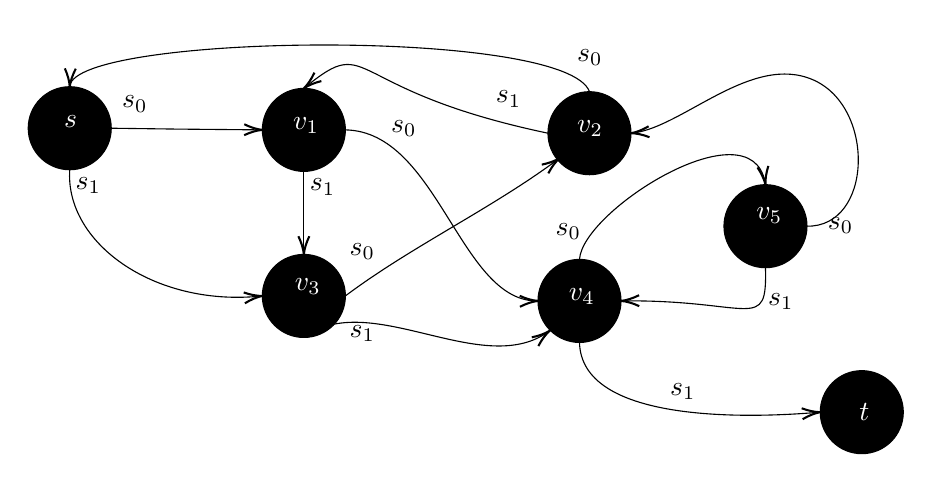
\begin{tikzpicture}[x=0.6pt,y=0.6pt,yscale=-1,xscale=1]
%uncomment if require: \path (0,300); %set diagram left start at 0, and has height of 300

%Shape: Circle [id:dp5495329281078569] 
\draw  [fill={rgb, 255:red, 0; green, 0; blue, 0 }  ,fill opacity=1 ] (32,49) .. controls (32,35.19) and (43.19,24) .. (57,24) .. controls (70.81,24) and (82,35.19) .. (82,49) .. controls (82,62.81) and (70.81,74) .. (57,74) .. controls (43.19,74) and (32,62.81) .. (32,49) -- cycle ;
%Straight Lines [id:da33331850965746734] 
\draw    (82,49) -- (121.98,49.53) -- (171,49.98) ;
\draw [shift={(173,50)}, rotate = 180.52] [color={rgb, 255:red, 0; green, 0; blue, 0 }  ][line width=0.75]    (10.93,-3.29) .. controls (6.95,-1.4) and (3.31,-0.3) .. (0,0) .. controls (3.31,0.3) and (6.95,1.4) .. (10.93,3.29)   ;
%Shape: Circle [id:dp8549825383964691] 
\draw  [fill={rgb, 255:red, 0; green, 0; blue, 0 }  ,fill opacity=1 ] (173,50) .. controls (173,36.19) and (184.19,25) .. (198,25) .. controls (211.81,25) and (223,36.19) .. (223,50) .. controls (223,63.81) and (211.81,75) .. (198,75) .. controls (184.19,75) and (173,63.81) .. (173,50) -- cycle ;
%Straight Lines [id:da15070581279870932] 
\draw    (198,75) -- (198,123) ;
\draw [shift={(198,125)}, rotate = 270] [color={rgb, 255:red, 0; green, 0; blue, 0 }  ][line width=0.75]    (10.93,-3.29) .. controls (6.95,-1.4) and (3.31,-0.3) .. (0,0) .. controls (3.31,0.3) and (6.95,1.4) .. (10.93,3.29)   ;
%Shape: Circle [id:dp4390825091110777] 
\draw  [fill={rgb, 255:red, 0; green, 0; blue, 0 }  ,fill opacity=1 ] (345,52) .. controls (345,38.19) and (356.19,27) .. (370,27) .. controls (383.81,27) and (395,38.19) .. (395,52) .. controls (395,65.81) and (383.81,77) .. (370,77) .. controls (356.19,77) and (345,65.81) .. (345,52) -- cycle ;
%Shape: Circle [id:dp9757305512769809] 
\draw  [fill={rgb, 255:red, 0; green, 0; blue, 0 }  ,fill opacity=1 ] (173,150) .. controls (173,136.19) and (184.19,125) .. (198,125) .. controls (211.81,125) and (223,136.19) .. (223,150) .. controls (223,163.81) and (211.81,175) .. (198,175) .. controls (184.19,175) and (173,163.81) .. (173,150) -- cycle ;
%Shape: Circle [id:dp6476109813645592] 
\draw  [fill={rgb, 255:red, 0; green, 0; blue, 0 }  ,fill opacity=1 ] (339,153) .. controls (339,139.19) and (350.19,128) .. (364,128) .. controls (377.81,128) and (389,139.19) .. (389,153) .. controls (389,166.81) and (377.81,178) .. (364,178) .. controls (350.19,178) and (339,166.81) .. (339,153) -- cycle ;
%Shape: Circle [id:dp9387189635111892] 
\draw  [fill={rgb, 255:red, 0; green, 0; blue, 0 }  ,fill opacity=1 ] (451,108) .. controls (451,94.19) and (462.19,83) .. (476,83) .. controls (489.81,83) and (501,94.19) .. (501,108) .. controls (501,121.81) and (489.81,133) .. (476,133) .. controls (462.19,133) and (451,121.81) .. (451,108) -- cycle ;
%Shape: Circle [id:dp6728900489022538] 
\draw  [fill={rgb, 255:red, 0; green, 0; blue, 0 }  ,fill opacity=1 ] (509,220) .. controls (509,206.19) and (520.19,195) .. (534,195) .. controls (547.81,195) and (559,206.19) .. (559,220) .. controls (559,233.81) and (547.81,245) .. (534,245) .. controls (520.19,245) and (509,233.81) .. (509,220) -- cycle ;
%Curve Lines [id:da06839655673782064] 
\draw    (223,50) .. controls (278.44,50.99) and (291.74,151.95) .. (337.6,153) ;
\draw [shift={(339,153)}, rotate = 178.78] [color={rgb, 255:red, 0; green, 0; blue, 0 }  ][line width=0.75]    (10.93,-3.29) .. controls (6.95,-1.4) and (3.31,-0.3) .. (0,0) .. controls (3.31,0.3) and (6.95,1.4) .. (10.93,3.29)   ;
%Curve Lines [id:da30024168681774177] 
\draw    (364,178) .. controls (364.99,225.52) and (461.05,224.04) .. (507.6,220.12) ;
\draw [shift={(509,220)}, rotate = 175.03] [color={rgb, 255:red, 0; green, 0; blue, 0 }  ][line width=0.75]    (10.93,-3.29) .. controls (6.95,-1.4) and (3.31,-0.3) .. (0,0) .. controls (3.31,0.3) and (6.95,1.4) .. (10.93,3.29)   ;
%Curve Lines [id:da031177664907863667] 
\draw    (370,27) .. controls (356.28,-11.22) and (69.81,-8.14) .. (57.41,22.11) ;
\draw [shift={(57,24)}, rotate = 271.79] [color={rgb, 255:red, 0; green, 0; blue, 0 }  ][line width=0.75]    (10.93,-3.29) .. controls (6.95,-1.4) and (3.31,-0.3) .. (0,0) .. controls (3.31,0.3) and (6.95,1.4) .. (10.93,3.29)   ;
%Curve Lines [id:da19551484489395188] 
\draw    (364,128) .. controls (365.79,98.44) and (466.95,34.79) .. (475.76,81.55) ;
\draw [shift={(476,83)}, rotate = 261.95] [color={rgb, 255:red, 0; green, 0; blue, 0 }  ][line width=0.75]    (10.93,-3.29) .. controls (6.95,-1.4) and (3.31,-0.3) .. (0,0) .. controls (3.31,0.3) and (6.95,1.4) .. (10.93,3.29)   ;
%Curve Lines [id:da5453571551089418] 
\draw    (345,52) .. controls (220.26,25.76) and (239.59,-8.8) .. (199.24,23.99) ;
\draw [shift={(198,25)}, rotate = 320.6] [color={rgb, 255:red, 0; green, 0; blue, 0 }  ][line width=0.75]    (10.93,-3.29) .. controls (6.95,-1.4) and (3.31,-0.3) .. (0,0) .. controls (3.31,0.3) and (6.95,1.4) .. (10.93,3.29)   ;
%Curve Lines [id:da7736997926226343] 
\draw    (223,150) .. controls (262.6,120.3) and (311.02,97.46) .. (350.8,67.9) ;
\draw [shift={(352,67)}, rotate = 143.13] [color={rgb, 255:red, 0; green, 0; blue, 0 }  ][line width=0.75]    (10.93,-3.29) .. controls (6.95,-1.4) and (3.31,-0.3) .. (0,0) .. controls (3.31,0.3) and (6.95,1.4) .. (10.93,3.29)   ;
%Curve Lines [id:da35489757719958615] 
\draw    (57,74) .. controls (54.03,117.56) and (106.93,156.22) .. (171.05,150.2) ;
\draw [shift={(173,150)}, rotate = 173.85] [color={rgb, 255:red, 0; green, 0; blue, 0 }  ][line width=0.75]    (10.93,-3.29) .. controls (6.95,-1.4) and (3.31,-0.3) .. (0,0) .. controls (3.31,0.3) and (6.95,1.4) .. (10.93,3.29)   ;
%Curve Lines [id:da7424500525745132] 
\draw    (198,175) .. controls (237.6,145.3) and (304.64,199.89) .. (344.79,171.87) ;
\draw [shift={(346,171)}, rotate = 143.13] [color={rgb, 255:red, 0; green, 0; blue, 0 }  ][line width=0.75]    (10.93,-3.29) .. controls (6.95,-1.4) and (3.31,-0.3) .. (0,0) .. controls (3.31,0.3) and (6.95,1.4) .. (10.93,3.29)   ;
%Curve Lines [id:da3132040250840804] 
\draw    (501,108) .. controls (540.44,108.6) and (542.5,36.73) .. (505,20) .. controls (468.25,3.6) and (426.87,47.76) .. (396.83,51.8) ;
\draw [shift={(395,52)}, rotate = 355.43] [color={rgb, 255:red, 0; green, 0; blue, 0 }  ][line width=0.75]    (10.93,-3.29) .. controls (6.95,-1.4) and (3.31,-0.3) .. (0,0) .. controls (3.31,0.3) and (6.95,1.4) .. (10.93,3.29)   ;
%Curve Lines [id:da9721751571878057] 
\draw    (476,133) .. controls (477,172.8) and (468.09,152.21) .. (390.18,152.99) ;
\draw [shift={(389,153)}, rotate = 359.27] [color={rgb, 255:red, 0; green, 0; blue, 0 }  ][line width=0.75]    (10.93,-3.29) .. controls (6.95,-1.4) and (3.31,-0.3) .. (0,0) .. controls (3.31,0.3) and (6.95,1.4) .. (10.93,3.29)   ;

% Text Node
\draw (87,28) node [anchor=north west][inner sep=0.75pt]   [align=left] {$\displaystyle s_{0}$};
% Text Node
\draw (52,40) node [anchor=north west][inner sep=0.75pt]  [color={rgb, 255:red, 255; green, 255; blue, 255 }  ,opacity=1 ] [align=left] {$\displaystyle s$};
% Text Node
\draw (59,77) node [anchor=north west][inner sep=0.75pt]   [align=left] {$\displaystyle s_{1}$};
% Text Node
\draw (249,43) node [anchor=north west][inner sep=0.75pt]   [align=left] {$\displaystyle s_{0}$};
% Text Node
\draw (190,41) node [anchor=north west][inner sep=0.75pt]  [color={rgb, 255:red, 255; green, 255; blue, 255 }  ,opacity=1 ] [align=left] {$\displaystyle v_{1}$};
% Text Node
\draw (200,78) node [anchor=north west][inner sep=0.75pt]   [align=left] {$\displaystyle s_{1}$};
% Text Node
\draw (361,0) node [anchor=north west][inner sep=0.75pt]   [align=left] {$\displaystyle s_{0}$};
% Text Node
\draw (361,43) node [anchor=north west][inner sep=0.75pt]  [color={rgb, 255:red, 255; green, 255; blue, 255 }  ,opacity=1 ] [align=left] {$\displaystyle v_{2}$};
% Text Node
\draw (224,117) node [anchor=north west][inner sep=0.75pt]   [align=left] {$\displaystyle s_{0}$};
% Text Node
\draw (191,138) node [anchor=north west][inner sep=0.75pt]  [color={rgb, 255:red, 255; green, 255; blue, 255 }  ,opacity=1 ] [align=left] {$\displaystyle v_{3}$};
% Text Node
\draw (224,166) node [anchor=north west][inner sep=0.75pt]   [align=left] {$\displaystyle s_{1}$};
% Text Node
\draw (348,105) node [anchor=north west][inner sep=0.75pt]   [align=left] {$\displaystyle s_{0}$};
% Text Node
\draw (356,144) node [anchor=north west][inner sep=0.75pt]  [color={rgb, 255:red, 255; green, 255; blue, 255 }  ,opacity=1 ] [align=left] {$\displaystyle v_{4}$};
% Text Node
\draw (417,201) node [anchor=north west][inner sep=0.75pt]   [align=left] {$\displaystyle s_{1}$};
% Text Node
\draw (512,101) node [anchor=north west][inner sep=0.75pt]   [align=left] {$\displaystyle s_{0}$};
% Text Node
\draw (469,95) node [anchor=north west][inner sep=0.75pt]  [color={rgb, 255:red, 255; green, 255; blue, 255 }  ,opacity=1 ] [align=left] {$\displaystyle v_{5}$};
% Text Node
\draw (476,147) node [anchor=north west][inner sep=0.75pt]   [align=left] {$\displaystyle s_{1}$};
% Text Node
\draw (531,213) node [anchor=north west][inner sep=0.75pt]  [color={rgb, 255:red, 255; green, 255; blue, 255 }  ,opacity=1 ] [align=left] {$\displaystyle t$};
% Text Node
\draw (312,25) node [anchor=north west][inner sep=0.75pt]   [align=left] {$\displaystyle s_{1}$};


\end{tikzpicture}

  \caption{An example instance of the arrival problem.}\label{arrivalDiagram}
\end{figure}
There is an obvious algorithm to solve the $\textsc{Arrival}$ problem;
just simulate the walk. However, the case of instances where $t$ is not reachable pose a problem.
If $t$ is not reachable, the walk must cycle infinitely and never terminate!
The following content demonstrates that this is a non issue.
\begin{definition}[Hopeful and Desperation]
  Let $(V, s, t, s_0, s_1)$ be an instance of the $\arr$ problem. A vertex $v \in V$
  is \emph{hopeful} if there is a path $v \to t$ in the directed graph defined with
  the vertex set $V$ the edge set $E \subseteq V \times V$ with $(u, v) \in E$ if and
  only if either $s_0(u) = v$ or $s_1(u) = v$. The \emph{desperation} of a hopeful vertex
  $v$ is the length of the shortest path from $v$ to $t$.
\end{definition}
\begin{lemma}[\citep{arrivalBasic}]
  Let $(V, s, t, s_0, s_1)$  be an instance of the $\arr$ problem. If $v \in V$ is hopeful,
  the arrival walk passes through $v$ at most $2^{|V|}$ times.
\end{lemma}
\begin{proof}
  Begin by noting that if a vertex is hopeful, it's desperation is at most $|V|$. I perform
  an induction on the desperation of $v$. Suppose the desperation of $v \in V$ is 1. Then either
  $s_0(v) = t$ or $s_1(v) = t$. If $s_0(v) = t$, $t$ will be reached after passing through $v$ once.
  If $s_1(v) = t$ and $s_0(v) \neq t$ $t$ will be reached after passing through $v$ twice. In
  both cases $v$ is passed through at most $2^1 = 2$ times. \\
  Suppose that all hopeful vertices with desperation $d - 1$ are passed through at most $2^{d-1}$ times.
  Then if $v \in V$ is hopeful with desperation $d$, for some hopeful $w \in V$ with desperation
  $d - 1$ either $s_0(v) = w$ or $s_1(v) = w$. So at least every second passing of $v$, the
  walk will proceed to $w$. But the walk can pass through $w$ at most $2^{d-1}$ times,
  so the walk can pass through $v$ at most $2 \cdot 2^{d - 1} = 2^d$ times.
\end{proof}
\begin{cor}\label{walkFinite}
  Let $(V, s, t, s_0, s_1)$ be an instance of the $\arr$ problem. Then the arrival
  walk either reaches $t$, or reaches a vertex which is not hopeful.
\end{cor}
From \cref{walkFinite} it is clear that deciding an instance of the $\arr$ problem is
equivalent to deciding whether or not the arrival walk reaches $t$ or reaches a vertex which
is not hopeful. 
\begin{definition}[Processed Arrival]
  Let $(V, s, t, s_0, s_1)$ be an instance of the arrival problem. Let
  $\sim$ be the equivalence relation on $V$ generated by $u \sim v$ if
  $u$ and $v$ are both not hopeful.
  The \emph{processed arrival problem}
  is a set of vertices $V' = V / \sim$, the canonical projections of $s, t, s_0, s_1$ into $V'$,
  and a choice of representative $\overline{t} \in V'$ of all the non hopeful vertices in $V$.
\end{definition}
The set of non hopeful vertices can be easily computed in linear time with a breadth first search
from $t$. From this point on I will therefore refer
to instances of the $\arr$ problem exclusively as tuples $(V, s, t, \overline{t}, s_0, s_1)$ 
constructed as above.
\begin{cor}[\citep{arrivalBasic}]
  Let $(V, s, t, \overline{t}, s_0, s_1)$ be an instance of the $\arr$ problem,
  and $n = |V|$. The time complexity of the $\arr$ problem is $O(n \cdot 2^n)$.
\end{cor}
\begin{proof}
  I reason that the arrival walk on the processed instance $(V, s, t, \overline{t}, s_0, s_1)$
  has it's walk length bounded by $O(n \cdot 2^n)$. Every vertex $v \in V$ with $v \neq \overline{t}$
  is hopeful with desperation at most $n$, so by \cref{walkFinite} can be passed through at most
  $2^{n}$ times. If the walk reaches $t$ or $\overline{t}$ it terminates, and there are at most
  $n$ vertices $w \in V$ such that $w \not\in \{t, \overline{t}\}$, so the walk can take at most
  $n \cdot 2^n$ steps.
\end{proof}
There are in fact instances of the $\arr$ problem with exponentially long walks. A diagram
of such a case can be seen in \cref{expLongArrival}.
\begin{figure}
  \caption{An arrival instance with an exponentially long walk.}\label{expLongArrival}
\end{figure}
\begin{definition}[Switching Flow]
  Let $(V, s, t, s_0, s_1)$ be an arrival graph. A \emph{switching flow} is a pair of maps 
  $f_0, f_1 : V \to V$ such that the following axioms hold.
  \begin{itemize}
    \item For all $v \in V$
  \end{itemize}
\end{definition}
Interestingly, the $\textsc{Arrival}$ problem is polynomial-time reducible to $\trsk$. 
This idea was used in \citep{gärtner2021subexponential} in a slightly different form to what is presented here
to give a sub-exponential time algorithm for solving the $\textsc{Arrival}$ problem. 
The rest of this section will be demonstrating the reduction from $\arr$ to $\trsk$.


\chapter{Your next chapter}

A dissertation usually contains several chapters.

\chapter{Conclusions}

\section{Final Reminder}

The body of your dissertation, before the references and any appendices,
\emph{must} finish by page~40. The introduction, after preliminary material,
should have started on page~1.

You may not change the dissertation format (e.g., reduce the font size, change
the margins, or reduce the line spacing from the default single spacing). Be
careful if you copy-paste packages into your document preamble from elsewhere.
Some \LaTeX{} packages, such as \texttt{fullpage} or \texttt{savetrees}, change
the margins of your document. Do not include them!

Over-length or incorrectly-formatted dissertations will not be accepted and you
would have to modify your dissertation and resubmit. You cannot assume we will
check your submission before the final deadline and if it requires resubmission
after the deadline to conform to the page and style requirements you will be
subject to the usual late penalties based on your final submission time.

% \bibliographystyle{plain}
\bibliographystyle{plainnat}
\bibliography{mybibfile}


% You may delete everything from \appendix up to \end{document} if you don't need it.
\appendix

\chapter{First appendix}

\section{First section}

Any appendices, including any required ethics information, should be included
after the references.

Markers do not have to consider appendices. Make sure that your contributions
are made clear in the main body of the dissertation (within the page limit).

\chapter{Participants' information sheet}

If you had human participants, include key information that they were given in
an appendix, and point to it from the ethics declaration.

\chapter{Participants' consent form}

If you had human participants, include information about how consent was
gathered in an appendix, and point to it from the ethics declaration.
This information is often a copy of a consent form.


\end{document}
